% =============================================================================
% sections/design/rover/ground_station_overview.tex  -  Ground Station Overview
% Teams: ground_station (best guess - unconfirmed) / Status: EXAMPLE (scope approximation)
%
% EXAMPLE CONTENT for scope/layout approximation - not final report text.
% Adapted from the Preliminary Report's "Ground Station Setup and
% Equipment" subsection, trimmed to minimal prose. Marked with \exampleflag
% on its heading in the assembler.
%
% Images are placeholders (teams/ground_station/figures/gs_*.png) - swap
% them for the real scheme/photo by overwriting the same files.
% =============================================================================

The Ground Station Unit (GSU) provides operators with real-time control,
data visualization, and status monitoring. Its core setup includes a
ground station PC for video decoding and telemetry, a user interface with
two monitors, a control panel, and a rover controller for manual
navigation, plus a tripod-mounted directional antenna connected via
Ethernet within a \qty{20}{\meter} radius, shown in
\autoref{fig:ground_station_setup}.

\begin{figure}[!htbp]
    \centering
    \setlength{\fboxsep}{0pt}

    \begin{minipage}[c]{0.49\textwidth}
        \centering
        
\includegraphics[height=3.5cm, keepaspectratio]{teams/ground_station/figures/gs_scheme}
    \end{minipage}
    \hfill
    \begin{minipage}[c]{0.49\textwidth}
        \centering
        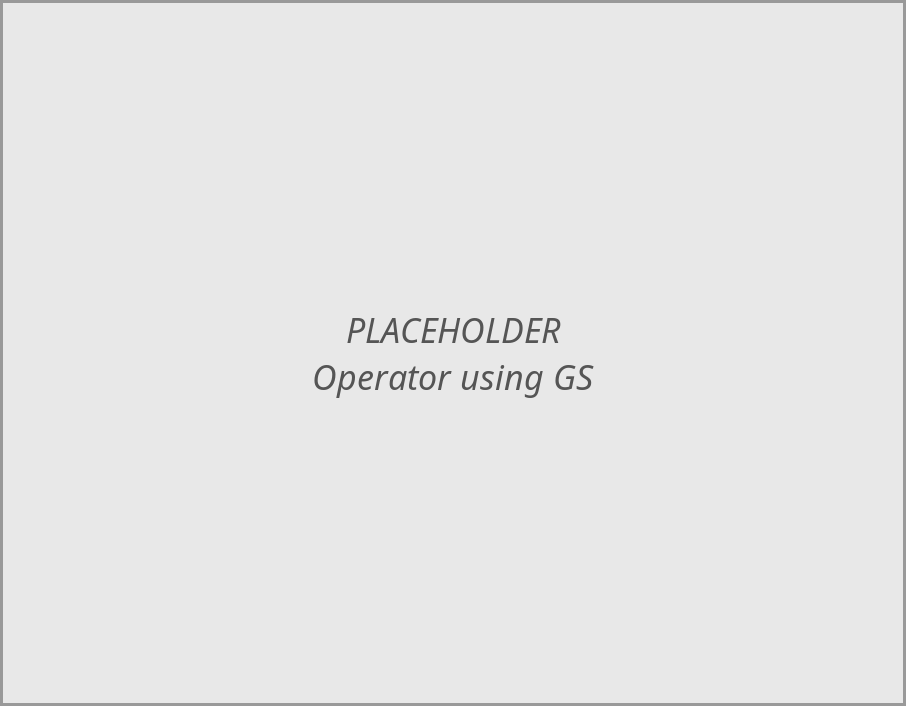
\includegraphics[height=3.5cm, keepaspectratio]{teams/ground_station/figures/gs_operator}
    \end{minipage}

    \caption{Ground Station Unit: scheme with sizes (left) and operator in use (right)}
    \label{fig:ground_station_setup}
\end{figure}
